\begin{ccRefFunctionObjectConcept}{Kernel::ConstructVertex_3}
A model for this must provide:

\ccCreationVariable{fo}

\ccMemberFunction{Kernel::Point_3 operator()(const Kernel::Segment_3
  &s, int i);} {returns source or target of \ccc{s}: \ccVar\ccc{(s,0)}
  returns the source of \ccc{s}, \ccVar\ccc{(s,1)} returns the target
  of \ccc{s}. The parameter \ccc{i} is taken modulo 2. }

\ccMemberFunction{Kernel::Point_3 operator()(const
  Kernel::Iso_cuboid_3 &c, int i);} {returns the i'th vertex of
  \ccc{c}, as indicated in the figure below. The parameter \ccc{i} is
  taken modulo 8. 
  \lcTex{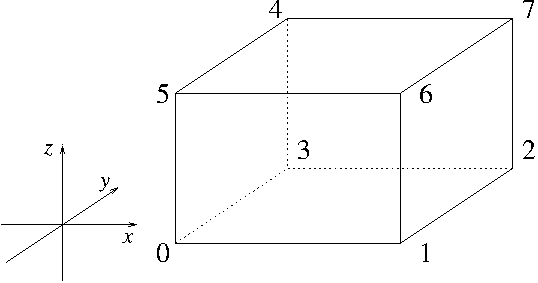
\includegraphics[width=6cm]{Kernel_23_ref/fig/IsoCuboid}}}

\begin{ccHtmlOnly}
<center>
<img border=0 src="fig/IsoCuboid.gif" align=middle 
  alt="vertex order of an iso-cuboid">
</center>
\end{ccHtmlOnly} 

\ccMemberFunction{Kernel::Point_3 operator()(const Kernel::Triangle_3
  &t, int i);} {returns the i'th vertex of \ccc{t}. The parameter
  \ccc{i} is taken modulo 3.}

\ccMemberFunction{Kernel::Point_3 operator()(const
  Kernel::Tetrahedron_3 &t, int i);} {returns the i'th vertex of
  \ccc{t}. The parameter \ccc{i} is taken modulo 4.}

\ccRefines
\ccc{AdaptableFunctor} (with two arguments)

\ccSeeAlso
\ccRefIdfierPage{CGAL::Iso_cuboid_3<Kernel>} \\
\ccRefIdfierPage{CGAL::Segment_3<Kernel>} \\
\ccRefIdfierPage{CGAL::Tetrahedron_3<Kernel>}  \\
\ccRefIdfierPage{CGAL::Triangle_3<Kernel>} \\

\end{ccRefFunctionObjectConcept}
